\documentclass[12 pt, a4paper]{article}
\usepackage[utf8]{inputenc}
\usepackage[margin={1 in}]{geometry}
\usepackage{amsfonts}
\usepackage{import}
\usepackage{color}
\usepackage{graphicx}
\graphicspath{{img/}}
%pag 801
\title{
	{Conocimiento en el aprendizaje}\\
	{\large Universidad Mayor de San Simón}\\
	{\large Intelligencia Artificial II}
}
\author{{Jose Enrique Camacho Silvestre}\and {Alexander Mamani Yucra}\and {Rudy Walter Martinez Melgarejo}}

\date{26 de mayo de 2020}

\begin{document}
	\maketitle
	\section{Antecedentes}
	Antes de poder explicar los distintos de métodos de aprendizaje es necesario poseer conocimientos previos de algunos conceptos, el objetivo de esta sección es presentarlos de manera superficial.
		\subsection{Aprendizaje inductivo}
			En nuestro enfoque definimos una función como un conjunto de pares ordenados.
			
			Sea \(f\) una función \(f: \mathbb{R} \mapsto \mathbb{R} \) y desconocida, \(f(x)\) el valor de la función \(f\) en \(x\), \(\mathcal{A}\) un conjunto tal que \(\mathcal{A} \subseteq f\),  devolver una función \(h\) denominada \emph{hipótesis} que se aproxime a la función \(f\) a partir del conjunto \(\mathcal{A}\). 
			
			Para este tipo de aprendizaje nos intersa pensar en una \emph{hipótesis} como un polinomio \(h := P(x)\). Un polinomio puede definirse de la siguiente manera:
			
			\begin{center}
				Sea \( n \in \mathbb{N}\), entonces \(P_{n}(x) =  \sum_{i = 0}^{n} a_{i}x^{i}\)
			\end{center}				
			\(H\) el conjunto de hipótesis a considerar denominado \emph{espacio de hipótesis}: 

			\begin{center}
				Sea \(j, k \in \mathbb{N}\),  \(j\leq k\), entonces \(H = \{ P_{0}(x), P_{1}(x), P_{2}(x), ... , P_{j}(x) \}\). 
			\end{center}
			
			\emph{Consistencia}, se dice que una hipotesis es consitente si verifica todos los puntos, es decir \(\mathcal{A} \subset h\). Sin embargo pueden exister más de dos hipotesis consitentes, la solución a esto nos la da \emph{la navaja de Ockham}, en donde nos sugiere elegir la hipótesis más sencilla.
			
			Pueden existir hipótesis que no son consitentes sin embargo permiten hacer mejores predicciones, estas funciones realizan una buean generalización. Esto nos dice que existe la posibilidad de que la función \(f\) sea no determinística.
			
		%\subsection{Árboles de decisión}	
			
			
		\subsection{Conocimiento \emph{a priori} y \emph{a posteriori}}
			Tipos de conocimiento \emph{a priori} (en latín: 'previo a') y \emph{a posteriori} (en latín: 'posterior a'), estos se clasifican dependiendo el grado de depenedencia que poseen con respecto a la experiencia.
			
			El conocimiento o justificación \emph{a priori} es independiente de la experiencia, es decir, que no se requiere de ninguna investigación para ser considerado como verdadero, solo basta con comprender el significado de los términos involucrados, por ejemplo: ``Si Wilhelm II reinó al menos cuatro días, entonces reinó más de tres días.''  
			
			El conocimiento o justificación \emph{a posteriori} depende de la experiencia, es decir, que se requirio de una observación previa para convencerse de que la preposición es verdadera, por ejemplo: ``Wilhelm II reinó de 1888 a 1918'' Esta proposition, si es cierta, se conoce como conocimiento \emph{a posteriori} ya que es un hecho empírico que no se puede conocer simplemente por la razón. 
				 
	%En esta sección se plantea hablar de las capitulos o tipos de aprendizajes anteriores, de una manera de anecdota, sencilla y general, y a la vez de dar una visión general de nuestro capítulo, hablando de lo que son la hipotesis, seguramente se recurrirá a enciclopedias.
	\section{Una formulación lógica del aprendizaje}
	%En esta sección se plantea en primer lugar brindar de todo el conocimiento de lógica de primer orden e hipotesis.
	
	%Es(x, planeta), ¿Y por qué se escribe Planeta(x)? 
	%¿Por qué se usa adjetivos juntos al verbo ser? Yo soy alto, Él es blanco, y en oraciónes como: El gato negro, El materialismo filosófico.
		Antes de nada debemos especificar la notación, definir algunos conceptos y recordar algunas ideas vistas en el capítulo anterior.
		
		La lógica de predicados esta fuertemente inspirada en la idea de función matemática.
		
		Un predicado es una expresión lingüística (ejem.: \(EsHombre(socrates)\)) que se puede conectar con una o varias otras expresiones para formar una oración o también llamada sentencia (ejem.: \(EsHombre(socrates) \land EsHombre(platon)\land ...\)).
		
		%Tomando la sentencia proposicional brindada por un árbol de decisión: ``Un predicado meta es verdadero para un objeto si y sólo si se alcanza una de las ramas que llevan a \emph{verdadero}.'' Codificando
		
		Para dar entender mejor el concepto de ejemplo recordemos la definición de ejemplo que nos brinda los árboles decisión booleano, donde un ejemplo consiste en un vector de atributos de entrada, \(X\), y un único valor de salida booleano \(y\), formalmente (\(X, y\)).
		
		\begin{figure}[h]
			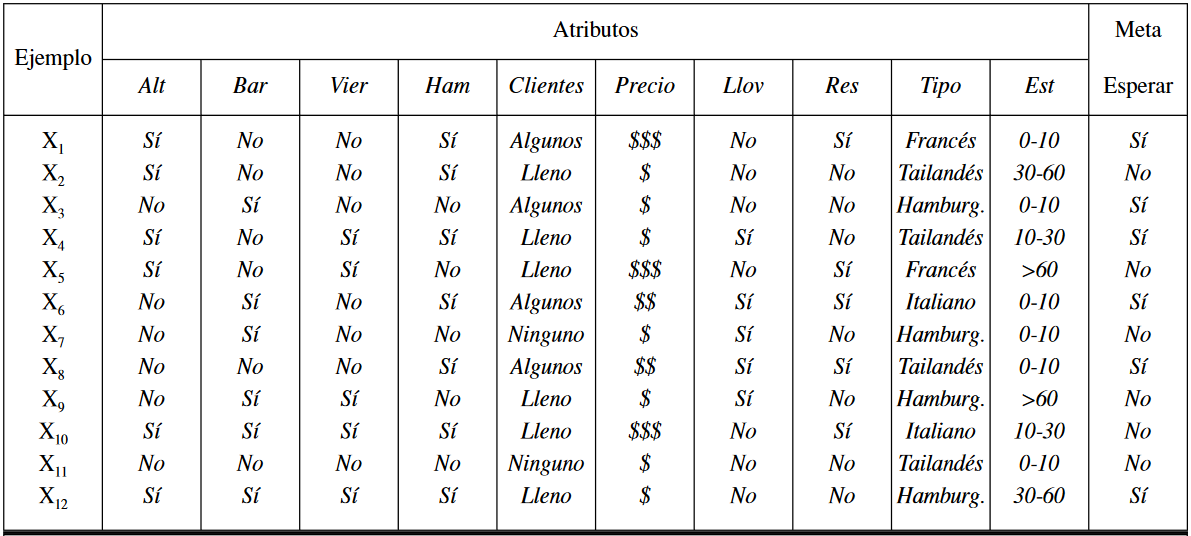
\includegraphics[width=\textwidth]{EjemploDT.png}
			\caption{Ejemplos para el dominio del restaurante}	
		\end{figure}
		Donde los ejemplos positivos son aquellos en los que la meta \(Esperar\) es verdadera, y los ejemplos negativos en los que es falsa. El conjunto de ejemplos completo se denomina \emph{conjunto de entrenamiento.}
		
		Esta definición de ejemplo no es la adecuada para este capítulo ya que aquí trabajamos con lógica de predicados, debído a esto en lugar de trabajar con un vector de atributos \(X\), nuestra entrada será una sentencia, donde los atributos se convertirán en predicados unarios, debido a esto ya no podemos pensar en nuestra entrada como ventor \(X\) más bien como una sentencia a la cual referenciaremos con \(E_{i}\) (entrada). Generalizando el ejemplo \(i\)-ésimo \(X_{i}\). Por ejemplo en el cuadro anterior, el primer ejemplo se describe a través de la sentencia:
			\[E_{1}:=Alternativa(X_{1}) \land \neg Bar(X_{1}) \land \neg Vier/Sab(X_{1}) \land Hambriento(X_{1}) \land ... \]
		
		\(D_{i}(X_{i})\) es una expresión cualquiera con unico argumento o aridad uno que representará el argumento de la entrada \(E_{i}\). El valor de salida del objeto \(E_{i}\) puede ser entedida como: La clasificación del objeto dada por la sentencia
			\[Esperar(X_{1})\]
			
		\(Q(X_{i})\) es una la notación genérica si el ejemplo es positivo, y \(\neg Q(X_{i})\) si el ejemplo es negativo. Esta notación generica es una sentencia que representa la salida del objeto \(E_{i}\) o mejor definida sentencia de clasificación o descripción. El conjunto completo de entrenamiento es la conjunción de todas las sentencias de descripción y clasificación.
		
		\textbf{Aprendizaje inductivo en el marco lógico} consiste en encontrar una expresión lógica equivalente al predicado meta \(Q\) con el objetivo de clasificar correctamente los ejemplos. Por \textbf{expresión lógica equivalente} al predicado meta \(Q\) nos referimos a una relación binaria a través del conectivo lógico de la doble implicación (\(\iff\)), esta relación no marca una relación fuerte que el lógica se denomina equivalente ya que si el antecedente es falso entonces el consecuente también es falso, y si el consecuente es verdadero el consecuente también los sera, es decir ambos tienen el mismo valor lógico. Por \textbf{clasificar correctamente los ejemplos} nos referimos a que dadas las entradas o sentencias \(E_{1}, E_{2},..,E_{i}\) la expresión econtrada debe darnos las salidas \(Q_{1},Q_{2},..,Q_{i}\). Cada \textbf{hipótesis} propone una expresión, que denominaremos una \textbf{definición candidata} del predicado meta. Usando \(C_{i}\) para representar la definición candidata, cada hipótesis \(h_{i}\) es una sentencia de la forma \(\forall x\quad Q(x) \iff C_{i}(x)\). En este punto conviene \emph{``separarnos''} un poco de la visión de función en la que veíamos nuestro formulación del aprendizaje y cabe centrarnos en la visión lógica, donde las entradas o \(E_{i}\), son sentencias que se tomarán como premisas verdaderas y nos servirán como base de conocimiento. 
		\begin{center}
			\textbf{Ejemplo:} Una hipótesis \(h_{r}\) pronene una definición candidata \(C_{r}\), la cual en lenguaje natural es: un predicado meta es verdadero para un objeto si y sólo si se alcanza una de las ramas que llevan a \emph{verdadero}. Formilazando esto en lógica:
		\end{center}
		\begin{figure}[h]
			\centering
			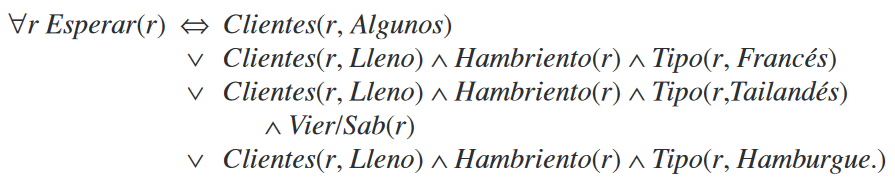
\includegraphics[width=0.9\textwidth]{candidateDefinition.png}
		\end{figure}

		Cada hipótesis predice que un cierto conjunto de ejemplos, es decir aquellos que satisfacen\footnote{Por satisfacer entendemos toda formula que es verdedara.} su definición candidata, serán ejemplos del predicado meta, en otras palabras toda \(C_{j}(x)\) de una hipotesis \(h_{j}\) que sea verdadero y que pertenezca al conjunto de ejemplos. Este conjunto se denomina \textbf{extensión} del predicado. Dos hipótesis con distintas extensiones son inconsistentes entre sí (\(\iff\)). Si tienen la misma extensión, son lógicamente equivalentes.
		\begin{figure}[hbt!]		
			\centering
			\import{img/}{set.pdf_tex}
			\caption{$\mathcal{A}$=Todas las posibles predicciones de $C_{j}$. $\mathcal{B}$=Predicciones positivas de $C_{j}$. $\mathcal{C}$= Predicciones de $C_{j}$ que forman parte del conjunto de ejemplos.}
			\label{fig: set_output}
		\end{figure}
		
		El espacio de hipótesis \(H\) es el conjunto de todas las hipótesis \(h_{1},..,h_{n}\) que el algoritmo de aprendizaje está diseñado para considerar. Se supone que el algoritmos de aprendizaje considera que una de la hipótesis es correcta:
		$$h_{1} \lor h_{2} \lor h_{3}\lor ... \lor h_{n}$$
		
		Podemos ir excluyendo las hipotesis que no son \emph{consistentes}, la no consitencia para un ejemplo puede ocurrir de dos formas:
		
		\begin{itemize}
			\item Un ejemplo puede ser \textbf{falso negativo} para la hipótesis, si la hipótesis afirma que debe ser negativo pero en realidad es positivo.\\
			\item Un ejemplo puede ser un \textbf{falso positivo} para la hipótesis, si la hipótesis afirma quedebe ser positivo pero en realidad es negativo.
		\end{itemize}
		
		Entonces un ejemplo puede ser incosistente con una hipotesis, podemos aprovechar esto para ir eliminando una o más hipotesis.
		 
		 Por lo tanto, podemos caracterizar el aprendizaje inductivo en un marco lógico como un proceso de eliminación gradual de las hipótesis que son incosistentes con los ejemplos, reduciendo así las probabilidades. Sin embargo pueden existir espacios de hipotesis enormes e incluso infinitos por eso describimos dos enfoques que encuentran hipótesis lógicamente con mucho menos esfuerzo.
		 
		 \subsection{Búsqueda mejor-hipótesis-actual}
			La idea de la búsqueda mejor-hipotesis-actual es mantener una única hipótesis, y ajustarla cuando llegan nuevos ejemplos para que se mantenga la consistencia.
			
			Supongamos que tenemos una hipótesis \(h_{r}\) cualquiera, y hasta el momento todos los ejemplos son consistentes. Donde el rectangulo es la extesión de \(h_{r}\). Entonces surge un ejemplo falso negativo, por lo tanto ese ejemplo debería formar parte de la extensión. La extensión debe \emph{aumentarse} e incluirlo. A esto se denomina \textbf{generalización}. Sin embargo surge otro ejemplo falso positivo, por lo tanto ese ejemplo no debería formar parte de la extensión. La extensión debe \emph{reducirse} y excluirla. A esto se denomina \textbf{especialización}.
				\begin{figure}[h]
					\centering
					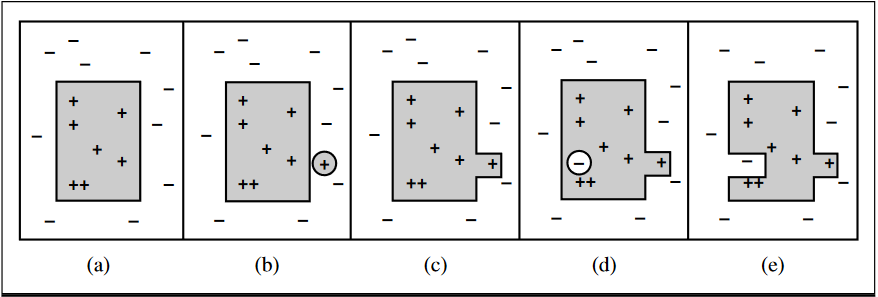
\includegraphics[width=0.9\textwidth]{SG.png}
				\end{figure}
			Ya en el algoritmo, tanto la espeficicación y generalización deben comprobar la consistencia con el resto de ejemplos.
			
				\begin{figure}[h]
					\centering
					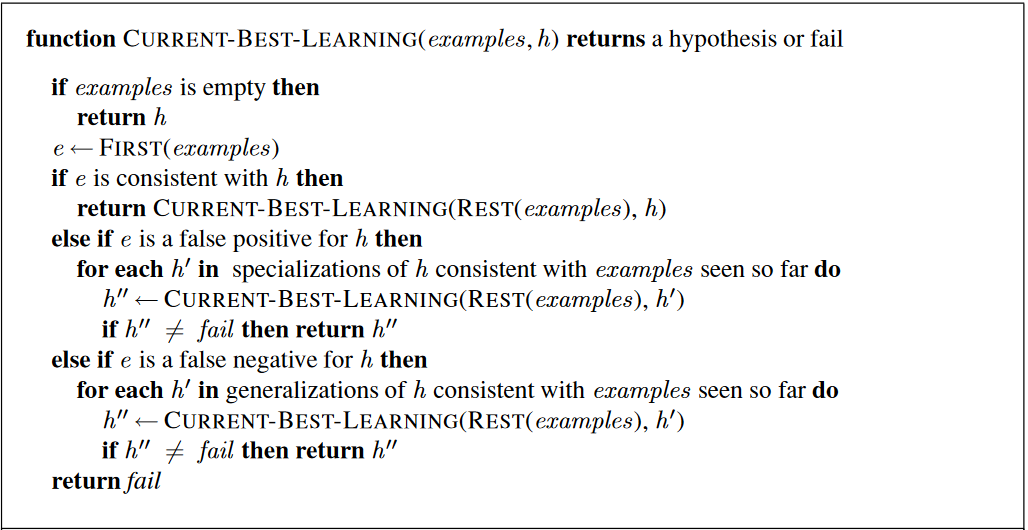
\includegraphics[width=0.9\textwidth]{BMHA_algorithm.png}
					\caption{Busca una hipótesis consistente que ajuste todos los ejemplos.}%pendiente.
				\end{figure}
			Entonces definimos la generalización y especialización como operaciones que cambian la \emph{extension} de nuestra hipótesis. Ahora necesitamos implementar operaciones sintácticas de manera exacta que modifiquen la definición candidata (\(C_{j}\)) asociada con la hipotesis. Esto se realiza observando que la generalización y la especialización son \textbf{realciones lógicas entre hipótesis}. Si la hipótesis $h_{1}$, con la definición $C_{1}$, es una generalización de la hipótesis $h_{2}$ con la definición $C_{2}$, entonces debemos tener
				$$\forall x\quad C_{2}(x) \Rightarrow C_{1}(x)$$
			Por lo tanto, para construir una generalización de $h_{2}$, necesitamos la definición $C_{1}$ que sea una implicación lógica de $C_{2}$. 
			
			Existen varias operaciones de gerneralización, pero el que usaremos será la \textbf{omisión de condiciones} (dropping conditions). Para especializar podemos \textbf{agregar condiciones} o \textbf{elimanar disyunciones} de una definición disyuntiva.
			
			\textbf{Ejemplo:} Usando la tabla de la figura 1, iremos construyendo nuestra hipotesis.
			\begin{itemize}
				\item El primer ejemplo $X_{1}$ es positivo. $Alternativa(X_{1})$ es verdadero, así que la hipótesis inicial será
					$$h_{1}: \forall x \quad Esperar(x) \Leftrightarrow Alternativa(x)$$
				\item El segundo ejemplo $X_{2}$ es negativo. $h_{1}$ lo predice como positivo, así que es un falso positivo. Por ello, tenemos que especializar $h_{1}$. Se puede hacer añadiendo una condición extra que rehace $X_{2}$. Una posibilidad es
					$$h_{2}: \forall x \quad Esperar(x) \Leftrightarrow Alternativa(x) \land Clientes(x, Algunos)$$
				\item  El tercer ejemplo $X_{3}$ es positivo. $h_{2}$ lo predice como negativo, luego es un falso negativo. Por ello, necesitamos generalizar $h_{2}$. Eliminamos la condición Alternativa, resultando
					$$h_{3}:\forall  x\quad Esperar(x) \Leftrightarrow Clientes(x, Algunos)$$
				\item El cuarto ejemplo $X_{4}$ es positivo. $h_{3}$ lo predice como negativo, luego es un falso negativo. Por ello, necesitamos generalizar. No podemos eliminar la condición de $Clientes$, ya que obtendríamos una hipótesis que incluye a todos los ejemplos,que sería inconsistente con $X_{2}$. Una posibilidad es añadir una disyunción:
					$$h_{4}:\forall x\quad Esperar(x) \Leftrightarrow Clientes(x, Algunos)\lor (Clientes(x, Lleno) \land Vier/Sab(x))$$
			\end{itemize}
				
				La hipótesis ya está comenzando a parecer razonable. Obviamente, existen otras posibilidades consistentes con los cuatro primeros ejemplos; aquí están otras dos:
					$$h_{4}':\forall x\quad Esperar(x) \Leftrightarrow \neg TiempoEsperaEstimado(x, 30-60)$$
					$$h_{4}'':\forall x\quad Esperar(x) \Leftrightarrow Clientes(x, Algunos)$$ 
					$$\lor (Clientes(x, Lleno) \land TiempoEsperaEstimado(x, 10-30))$$
			Este tipo de algoritmo es muy caro computacionalmente debido al \emph{backtraking}, se dice que es doblemente exponencial.
			
		%\subsection{Búsqueda de mínimo compromiso}
			
%%%%%%%%%%%%%%%%%%%%%%%%%%%%%%%%%%%%%%
	\section{Conocimiento en el aprendizaje}
	 	\subsection{Aprendizaje con conocimiento básico}
	 		El aprendizaje inductivo se basa en el descubrimiento de patrones a partir de ejemplos.
			
			El conocimiento a priori es aquel que, en algún sentido importante, es independiente de la experiencia.Para entender el papel del conocimiento a priori, necesitamos hablar de las relaciones lógicas entre hipótesis, descripciones de ejemplos y clasificaciones.
			
			\textbf{Descripciones:} Conjunción de todas las descripciones de los ejemplos del conjunto de entrenamiento.
			
			\textbf{Clasificaciones:} Conjunción de todas las clasificaciones de los ejemplos.
De este modo, las Hipótesis que ``explican las observaciones'' deben satisfacer la siguiente propiedad:
				
				\begin{figure}[h]
					\centering
					\includegraphics[width=0.6\textwidth]{./section2/fig1.png}
				\end{figure}
			
			Esta relación se denomina restricción, donde Hipótesis es lo ``desconocido''.  El objetivo del aprendizaje inductivo puro es resolver esta restricción, donde Hipótesis se obtiene a partir de algún espacio de hipótesis predefinido.
			
			Para construir un \emph{agente de aprendizaje autónomo que utilice conocimiento básico}, el agente debe contar con algún método para obtener el conocimiento básico, para que este conocimiento se pueda utilizar en los nuevos episodios de aprendizaje. Este método también debe ser en sí mismo un proceso de aprendizaje, la historia de la vida del agente estará caracterizada por un desarrollo acumulativo o incremental.
				\begin{figure}[h]
					\centering
					\includegraphics[width=0.85\textwidth]{./section2/fig2.png}
				\end{figure}
		\subsection{Ejemplos de aprendiaje con conocimiento básico}
			\subsubsection{Aprendizaje basado en explicaciones (EBL)}
			Ejemplo: Un hombre primitivo, está asando un lagarto en una vara. Es observado por una multitud asombrada de sus contemporáneos menos intelectuales, quienes han venido utilizando sus manos desnudas para mantener sus provisiones sobre el fuego. Esta instructiva experiencia es suficiente para convencer a los observadores de un principio general para cocinar sin dolor.
			
			Tipo de restricción: El hombre primitivo generaliza explicando el éxito de la vara: ésta soporta al lagarto, manteniendo así la mano lejos del fuego. A partir de esta explicación, infiere una \emph{regla general}: que cualquier objeto largo, rígido y puntiagudo sirve para asar alimentos pequeños y ligeros.
			
			Este tipo de proceso de generalización es denominado aprendizaje basado en explicaciones, o EBL (Explanation Based Learning). La regla general se deduce lógicamente del conocimiento básico que posee el hombre primitivo. Por lo tanto, las restricciones que se satisfacen por el EBL son las siguientes:
				\begin{figure}[h]
					\centering
					\includegraphics[width=0.6\textwidth]{./section2/fig3.png}
				\end{figure}
			
			EBL necesita que exista suficiente conocimiento básico como para explicar la Hipótesis, que en realidad explica las observaciones, por tanto, realmente el agente no aprende nada nuevo del ejemplo. El agente podría haber derivado el ejemplo de lo que ya sabía, aunque esto requiriera una cantidad muy elevada de computación. EBL no se considera como un método para convertir los primeros principios de las teorías en conocimiento útil de propósito específico.
			\subsubsection{Aprendizaje basado en Relevancia (RBL)}
			Ejemplo: Un turista va a Brasil y conoce a su primera persona brasileña. Al escucharle hablar en portugués, inmediatamente concluirá que los brasileños hablan en portugués, aunque al descubrir que su nombre es Fernando no concluirá que todos los brasileños se llaman Fernando.
			
			En este caso, el conocimiento a priori relevante es que, en cualquier país, la mayoría de la gente habla el mismo idioma; por otro lado, no se asume que Fernando sea el nombre de todos los brasileños, porque este tipo de regularidad no se verifica para los nombres.

			En este caso, el Conocimiento Básico a priori se refiere a la relevancia que tiene un conjunto de características sobre el predicado meta. Este conocimiento, junto con las observaciones, permite al agente inferir una nueva regla general que explica las observaciones:
				\begin{figure}[h]
					\centering
					\includegraphics[width=0.8\textwidth]{./section2/fig4.png}
				\end{figure}
			
			Como el RBL no hace uso del contenido de las observaciones, no produce hipótesis que vayan más allá del contenido lógico del conocimiento básico y de las observaciones. Es un método de aprendizaje deductivo, y por sí mismo no puede justificar la creación de nuevo conocimiento sin un conocimiento inicial de partida.
			
			\subsubsection{Aprendizaje inductivo basado en el conocimiento (Algoritmo KBIL)}
			\textbf{Ejemplo:} Un estudiante de Medicina sabe realizar diagnósticos sofisticados, pero es ignorante respecto a farmacología, está observando la consulta entre un paciente y un experto. Después de una serie de preguntas y respuestas, el experto dice al paciente que tome un determinado antibiótico. El estudiante de medicina inferirá la regla general sobre qué antibiótico particular es efectivo para un tipo de infección determinado.
			
			Se asume que el conocimiento a priori del estudiante es suficiente para inferir la enfermedad ($D$) del paciente a partir de los síntomas. Sin embargo, esto no es suficiente para explicar el hecho de que el doctor prescribe una medicina concreta ($M$) El estudiante necesita obtener otra regla: que $M$, generalmente, es una medicina efectiva contra la enfermedad $D$. Dada esta regla, y el conocimiento a priori con el que cuenta el estudiante, éste puede explicar por qué el experto prescribe $M$ en ese caso particular. Podemos generalizar este ejemplo para proponer la restricción:
				\begin{figure}[h]
					\centering
					\includegraphics[width=1\textwidth]{./section2/fig5.png}
				\end{figure}
			
	 \section{Aprendizaje basado en explicaciones}
	 		El aprendizaje basado en explicaciones es un método para extraer reglas generales a partir de observaciones particulares.
	 			\begin{figure}[h]
					\centering
					\includegraphics[width=0.8\textwidth]{./section2/fig6.png}
				\end{figure}
	 		Supongamos que estamos aprendiendo a integrar. Sabemos las reglas de integración, la tabla de integrales inmediatas y los métodos que podemos usar para resolverlas. Al principio, cuando nos dan una integral para resolver, vamos probando métodos hasta encontrar uno que nos de la solución de forma sencilla. Esto es, si decidimos aplicar un método y este nos lleva a una expresión más complicada, lo descartamos y probamos con otro. A medida que aumentamos nuestra experiencia en la resolución de integrales sabremos a simple vista cuál es el método más apropiado para obtener la solución. Un método EBL puede asociarse a un sistema de resolución de problemas de manera que nos permitirá aprender reglas de control que mejorarán su eficiencia
	 			\begin{figure}[h]
					\centering
					\includegraphics[width=0.8\textwidth]{./section2/fig7.png}
				\end{figure}
	 		\subsection{Técnicas de la memorización}
	 		La técnica de memorización ha sido extensamente utilizada en informática para acelerar los programas guardando los resultados de la computación. La idea básica de las funciones memo es acumular una base de datos de pares \emph{entrada/salida}; cuando se hace una llamada a la función, ésta, en primer lugar, comprueba la base de datos para ver si se puede evitar que la resolución del problema parta de cero.
	 		
	 		\subsection{Extracción de reglas generales a partir de ejemplos:}
			La idea en la que se basa EBL consiste en construir, en primer lugar, una explicación de la observación, utilizando conocimiento a priori, y posteriormente, establecer una definición de la clase de casos para los que se puede utilizar la misma estructura de explicación. Esta definición proporciona las bases para una regla que cubra todos los casos en la clase. La ``explicación'' puede ser una prueba lógica, aunque de forma más general, puede ser cualquier proceso de razonamiento o de resolución de problemas cuyos pasos estén bien definidos. La clave es ser capaz de identificar las condiciones necesarias para que los mismos pasos se puedan aplicar a otro caso.
			
			\subsection{Encadenamiento hacia atrás}
			El proceso de desarrollo de un Sistema basado en encadenamiento hacia atrás está dado de la siguiente manera:

			\begin{itemize}
				\item Se comienza con una meta para probar\\
				\item Se inspecciona la memoria de trabajo para ver si la meta ha sido     previamente probada\\
				\item En caso de que no se haya probado, el sistema busca en sus reglas para ver si     una o más tienen esta meta en su parte del \emph{THEN}, este tipo de regla     es llamada regla meta.\\
				\item El sistema ve si las premisas de las reglas meta están listadas en la memoria     de trabajo, las premisas no listadas se tornan nuevas metas o     subtemas para ser probadas.\\
				\item Este proceso continúa de manera recursiva hasta que el sistema encuentra una     premisa que no es soportada por ninguna regla, llamada primitiva     (premisa de una regla que no es concluida por ninguna regla)\\
				\item Cuando una primitiva es encontrada, el sistema pregunta al usuario información     acerca de esta primitiva, entonces el sistema usa esta información     para ayudar a probar los subtemas y la meta original\\
			\end{itemize}	
				\begin{figure}[h]
					\centering
					\includegraphics[width=0.6\textwidth]{./section2/fig8.png}
				\end{figure}
			
			En el encadenamiento hacia atrás, el orden a probar la hipótesis h deberá de probarse al menos una de las hipótesis intermedias. Se observa que el diagrama, en este caso se describe como un diagrama \emph{AND/OR} para indicar que en algún caso, tal como $h_{2}$ todas las hipótesis de nivel inferior deben estar presentes para sostener $h_{2}$.
	
			En otros casos, tal como la hipótesis de nivel superior $h$ solo es necesario una hipótesis de nivel inferior para que se verifique.En el encadenamiento hacia atrás, el sistema, por lo general, obtendrá evidencia del usuario, con el fin de probar o no la hipótesis, lo que contrasta con el sistema de encadenamiento hacia adelante, en el que todos los hechos relevantes se conocen por lo general con antelación.
			\subsubsection{Ejemplo del ecadenamiento hacia atrás}
			Supongamos que un paciente va al doctor, el doctor luego de escuchar el problema del paciente creé que tiene una infección de garganta. Ahora bien veremos como un sistema experto basado en reglas de encadenamiento hacia atrás puede solucionar este problema.
			
			\subsection{Proceso básico de EBL}
			El proceso básico de EBL funciona de la siguiente forma:
				\begin{enumerate}
						\item Dado un ejemplo, se construye una prueba para el predicado meta que se aplica al ejemplo, utilizando el conocimiento básico disponible.\\
						  \item En paralelo, se construye un árbol de prueba generalizado para la meta variabilizada, utilizando los mismos pasos de inferencia que en la prueba original.\\
						  \item Se construye una nueva regla cuya parte izquierda está formada por las hojas del árbol de prueba y cuya parte derecha es la meta variabilizada (después de aplicar las asignaciones necesarias de la prueba generalizada).\\
						  \item Se eliminan todas las condiciones que son verdaderas independientemente de los valores de las variables de la meta.\\
				\end{enumerate}
%%%%%%%%%%%%%%%%%%%%%%%%%%%%%%%%%%%%%%%%%%%%%%%%%%%%%%%%%%%%%%%%%%%%%%%%%%%%%%%%%
	 \section{Aprendizaje basado en información relevante}
		Parece que nuestro turista en Brasil es capaz de hacer una generalización segura sobre el idioma que hablan otros brasileños. 

		Su conocimiento básico autoriza la inferencia: la gente del mismo país (normalmente) habla el mismo idioma. Esto se puede expresar en lógica de primer orden de la siguiente manera:
		
			$$Nacionalidad(x, n) \land Nacionalidad(y, n) \land Idioma(x, l) \Rightarrow Idioma(y, l)$$
		
		No es difícil demostrar que a partir de esta sentencia y de la observación, 
		
			$$Nacionalidad(Fernando, Brasil) \land Idioma(Fernando, Portugues)$$
		
		Se deduce la siguiente conclusión:
		
			$$Nacionalidad(x, Brasil) \land Idioma(x, Portugues)$$
		Las sentencias anteriores expresan una forma estricta de relevancia: dada una nacionalidad, el idioma queda totalmente determinado. 
		
		Estas sentencias se denominan dependencias funcionales o determinaciones. Son tan comunes en algunos tipos de aplicaciones, que se utiliza una sintaxis especial para escribirlas. Adoptaremos la notación de Davies (1985):
		
			$$Nacionalidad(x, n)\succ Idioma(x, l)$$
		Esto es simplemente el azúcar sintáctico al que ya estamos acostumbrados, pero deja claro que la determinación es realmente una relación entre los predicados: la nacionalidad determina el lenguaje. 

		Las propiedades relevantes que determinan la conductancia y la densidad se pueden expresar de una forma similar:
			$$Material(x, m)\land Temperatura(x, t) \succ Conductancia(x, p);$$
			$$Material(x, m) \land Temperatura(x, t) \succ Densidad(x, d)$$
		
		\subsection{Determinar el espacio de hipótesis}
			Aunque las determinaciones autorizan la obtención de conclusiones generales para todos los brasileños, o para todas las piezas de cobre a una temperatura dada, por supuesto, no pueden dar lugar a una teoría de predicción general para todas las nacionalidades, o para todas las temperaturas y materiales, a partir de un simple ejemplo. 
			
			Se puede decir que su principal efecto es que limitan el espacio de hipótesis que el agente de aprendizaje necesita considerar. Por ejemplo, para predecir la conductancia, se necesita considerar únicamente el material y la temperatura, y se puede ignorar la masa, el propietario, el día de la semana, el presidente actual, etc. Desde luego, las hipótesis pueden incluir términos que vienen determinados por el material y la temperatura, como la estructura molecular, la energía térmica, o la densidad de electrones libres. Las determinaciones especifican un vocabulario básico suficiente para construir hipótesis relativas al predicado principal. Esta sentencia se puede demostrar mostrando que una determinación dada es lógicamente equivalente a una sentencia en la que el predicado principal es uno de los elementos del conjunto de todas las definiciones que se pueden expresar utilizando los predicados de la parte derecha de la determinación.
			
		\subsection{Aprender y utilizar información relevante}
			Como ya comentamos en la introducción de este capítulo, el conocimiento a priori es muy útil para el aprendizaje, pero también tiene que aprenderse. 
			
			Por lo tanto, para conocer completamente el aprendizaje basado en información relevante, debemos proporcionar un algoritmo de aprendizaje para determinaciones. El algoritmo de aprendizaje que vamos a presentar se basa en un intento sencillo para encontrar la determinación más simple que es consistente con las observaciones. Una determinación $P \succ Q$ indica que si algunos ejemplos encajan con $P$, también deben encajar con $Q$. Por lo tanto, una determinación es consistente con un conjunto de ejemplos, si cada par que encaja con los predicados de la parte izquierda también encaja con el predicado principal, es decir, tiene la misma clasificación. Por ejemplo, suponga que tenemos los siguientes ejemplos, relativos a medidas de conductancia en unas muestras de material:	
				\begin{figure}[h]
					\centering
					\includegraphics[width=0.85\textwidth]{./section3/fig1.png}
				\end{figure}
				
			La determinación consistente mínima es 
				$$Material \land Temperatura \succ Conductancia$$
			Existe una determinación no mínima, pero consistente: 
			$$Masa \land \textit{Tamaño} \land Temperatura \succ Conductancia$$
			Es consistente con los ejemplos porque la masa y el tamaño determinan la densidad, y en nuestro conjunto de datos no tenemos dos materiales diferentes con la misma densidad. Como es usual, necesitaríamos una muestra más grande para eliminar una hipótesis casi correcta.
				\begin{figure}[h]
					\centering
					\includegraphics[width=0.9\textwidth]{./section3/fig2.png}
				\end{figure}
			
	 \section{Programación lógica inductiva}
	 	Combina los métodos de inducción con la potencia de las representaciones de primer orden.
	 	
	 	\textbf{¿Por qué es tan popular?}
	 		\begin{itemize}
	 			\item Ofrece un enfoque riguroso al problema de aprendizaje inductivo basado en el conocimiento.\\
	 			\item Ofrece algoritmos completos para inducir teorías de primer orden generales, a partir de los ejemplos.\\
	 			\item Produce hipótesis que son (relativamente) fáciles de entender por humanos.\\
	 		\end{itemize}
	 		\textbf{Ejemplo:} Tenemos el problema general de inducción basado en el conocimiento cuyo fin es ``resolver'' la restricción.			
	 		$$\textit{ConocimientoBásico} \land \textit{Hipótesis}\land Descripciones \models Clasificaciones$$
	 		
	 		Para la \textbf{\textit{Hipótesis}} desconocida, dados el \textbf{\textit{ConocimientoBásico}} y los ejemplos descritos por las \textbf{\textit{Descripciones}} y las \textbf{\textit{Clasificaciones}}. 
	 		
	 		Para ilustrar esto, usaremos el problema de aprendizaje de relaciones familiares a partir de ejemplos.
	 		\begin{figure}[h]
					\centering
					\includegraphics[width=1\textwidth]{./section3/fig3.png}
				\end{figure}
			Las \textbf{\textit{Descripciones}} consistirán en un árbol genealógico extendido, descrito en términos de Madre, Padre, la relación CasadoCon y las propiedades Hombre y Mujer. 	
				\begin{figure}[h]
					\centering
					\includegraphics[width=0.8\textwidth]{./section3/fig4.png}
				\end{figure}
			Las sentencias en \textbf{\textit{Clasificaciones}} dependen del concepto objetivo que está siendo aprendido. 
Podríamos querer aprender $Abuelo/a$, \textit{Cuñado}, o \textbf{Ancestro}, por ejemplo. 
				\begin{figure}[h]
					\centering
					\includegraphics[width=0.8\textwidth]{./section3/fig5.png}
				\end{figure}
			Podríamos aprender a partir de un subconjunto de este conjunto completo.
	
			El objetivo de un programa de aprendizaje inductivo es proponer un conjunto de sentencias para la Hipótesis, tal que la restricción se satisfaga. 
			
			Suponga, por el momento, que el agente no tiene conocimiento básico: ConocimientoBásico es vacío. Entonces una posible solución para la Hipótesis es la siguiente:
				\begin{figure}[h]
					\centering
					\includegraphics[width=0.8\textwidth]{./section3/fig6.png}
				\end{figure}
				
			\textbf{Nóta:} Un algoritmo de aprendizaje basado en atributos, tal como \textbf{APRENDIZAJE - ÁRBOL -DECISIÓN}, no conseguirá nada a la hora de resolver este problema. Para poder expresar $Abuelo/a$ como un atributo (es decir, un predicado unario), necesitamos convertir pares de personas en objetos:
				$$Abuelo/a(<Mum, Charles>) ...$$
			Luego nos atascaremos intentando representar las descripciones del ejemplo. Los únicos atributos posibles tienen un aspecto tan horroroso como
				$$PrimerElementoEsMadreDeElisabeth(<Mum, Charles>)$$
			La definición de $Abuelo/a$ en términos de estos atributos simplemente se convierte en una gran disyunción de casos específicos que no generaliza para nuevos ejemplos. 
Los algoritmos de aprendizaje basados en atributos son incapaces de aprender predicados relacionales. 
Por ello, una de las principales ventajas de los algoritmos de ILP es su aplicabilidad a un mayor rango de problemas, incluyendo problemas de relaciones.

			Un poco de conocimiento básico ayudaría en la representación de la definición de $Abuelo/a$. Por ejemplo, si ConocimientoBásico incluye la sentencia
				$$Progenitor(x,y) \Leftrightarrow [Madre(x , y) \lor Padre(x, y)]$$
			entonces la definición de Abuelo/a se reduciría a
				$$Abuelo/a(x, y)\Leftrightarrow [\exists z \quad Progenitor(x, z) \land Progenitor(z, y)]$$
			
			Esto muestra cómo el conocimiento básico puede reducir considerablemente el tamaño de la hipótesis requerido para explicar las observaciones.

			Para los algoritmos de ILP también es posible crear nuevos predicados para expresar más fácilmente la hipótesis explicativa. Dado el ejemplo de datos mostrado anteriormente, es razonable para el programa ILP proponer un predicado adicional, al que llamaremos ``Progenitor'', para simplificar las definiciones de los predicados meta. Los algoritmos que pueden generar nuevos predicados se denominan algoritmos de inducción constructiva. 
			\subsection{Métodos de aprendizaje inductivo de arriba a abajo (Top-down)}
				Los primeros enfoques en trabajos de ILP comienzan con una regla muy general que gradualmente se especializa hasta que encaja con los datos. Esto es esencialmente lo que ocurre en el aprendizaje de árboles de decisión, donde se construye incrementalmente un árbol de decisión hasta que es consistente con todas las observaciones. 

				Para ILP usamos literales de primer orden en vez de atributos, y la hipótesis es un conjunto de cláusulas en vez de un árbol de decisión. 

				Suponga que estamos intentando aprender la definición de Abuelo(x,y), usando los mismos datos familiares que antes. Al igual que el aprendizaje de árboles de decisión, podemos dividir los ejemplos en positivos y negativos. 

				Los ejemplos positivos son
					$$<George, Anne>, <Philip, Peter>, <Spencer, Harry>, ...$$
				y los ejemplos negativos son
					$$<George, Elizabeth>, <Harry, Zara>, <Charles, Philip>, ...$$
				
				Nótese que cada ejemplo es un par de objetos, ya que Abuelo es un predicado binario.

				Existen 12 ejemplos positivos en el árbol genealógico y 388 ejemplos negativos (todos ellos pares de personas).

				FOIL construye un conjunto de cláusulas, cada una con $Abuelo(x,y)$ en la cabeza. Las cláusulas deben clasificar los 12 ejemplos positivos como instancias de la relación $Abuelo(x,y)$, y desechar los 388 ejemplos negativos. Las cláusulas son cláusulas de Horn, extendidas con literales negados usando la negación como fallo, al igual que en Prolog. La cláusula inicial tiene cuerpo vacío:
				
					$$\Rightarrow Abuelo(x,y)$$
				
				Esta cláusula clasifica todos los ejemplos como positivos, así que necesita ser especializada. Hacemos esto añadiendo literales a su parte izquierda, de uno en uno. A continuación se muestran tres adiciones posibles:
					$$Padre(x, y) \Rightarrow Abuelo(x, y)$$
					$$Progenitor(x, z) \Rightarrow Abuelo(x, y)$$
					$$Padre(x, z)\Rightarrow Abuelo(x, y)$$
				(Nótese que estamos asumiendo que una cláusula que define Progenitor forma parte del conocimiento básico.) 
				
				\begin{itemize}
					\item La primera de estas tres cláusulas clasifica incorrectamente todos los 12 ejemplos como negativos, así que puede ser ignorada.\\
					\item La segunda y la tercera clasifican correctamente los ejemplos positivos, pero la segunda es incorrecta con una gran parte de los ejemplos negativos (dos veces como mucho, ya que permite tanto madres como padres).\\
					\item Luego, preferiremos la tercera cláusula.\\
				\end{itemize}	
				Ahora, necesitamos especializar más la cláusula, para desechar los casos en los que $x$ es el padre de $z$, pero $z$ no es el progenitor de $y$. Añadiendo el literal $Progenitor(z,y)$ obtenemos
				
					$$Padre(x, z) \land Progenitor(z, y) \Rightarrow Abuelo(x, y)$$
					
				que clasifica correctamente todos los ejemplos. FOIL encontrará y elegirá este literal, resolviendo la tarea de aprendizaje. En general, FOIL tendrá que buscar en muchas cláusulas sin éxito antes de encontrar la solución correcta.
				\begin{figure}[h]
					\centering
					\includegraphics[width=0.9\textwidth]{./section3/fig7.png}
				\end{figure}
		\subsection{Aprendizaje inductivo con deducción inversa}
		La resolución inversa se basa en la observación de que si el ejemplo Clasificaciones resulta de \textbf{\textit{ConocimientoBásico $\land$ Hipótesis $\land$ Restricciones}}, entonces se puede probar este hecho a través de resolución. Si podemos ``ejecutar la prueba hacia atrás'', podemos encontrar una hipótesis tal que la prueba llegue a ella. La clave es encontrar una forma de invertir el proceso de resolución.	
		
		Mostraremos un proceso de prueba hacia atrás para la resolución inversa que consiste en pasos hacia atrás individuales. 
Recordando que un proceso normal de resolución toma dos cláusulas $C_{1}$ y $C_{2}$ y las resuelve produciendo el resolvente $C$.
Un paso de resolución inversa toma un resolvente $C$ y produce dos cláusulas $C_{1}$ y $C_{2}$, tal que $C$ es el resultado de resolver $C_{1}$ y $C_{2}$. 
	
		De forma alternativa, se podría tomar un resolvente C y una cláusula $C_{1}$ y producir una cláusula $C_{2}$ de forma que C es el resultado de resolver $C_{1}$ y $C_{2}$.
			\begin{figure}[h]
					\centering
					\includegraphics[width=0.8\textwidth]{./section3/fig8.png}
				\end{figure}		
		En esta figura se muestran los primeros pasos del proceso de resolución inversa, donde nos centramos en el ejemplo positivo $Abuelo/a(George, Anne)$. 
		
		El proceso comienza al final de la prueba.
Tomamos el resolvente $C$ como la cláusula vacía (es decir, una contradicción) y $C_{2}$ como $\neg Abuelo/a(George, Anne)$, que es la negación del ejemplo meta. 

		El primer paso inverso toma C y $C_{2}$ y genera la cláusula Abuelo/a(George, Anne) para $C_{1}$. 
		
		El siguiente paso toma esta cláusula como C y la cláusula $Progenitor(Elizabeth, Anne)$ como $C_{2}$, y genera la cláusula
			$$\neg Progenitor(Elizabeth, y) \lor Abuelo/a(George,y)$$

		como $C_{1}$. El último paso trata esta cláusula como resolvente. Con $Progenitor(George,Elizabeth)$ como $C_{2}$ , una posible cláusula $C_{1}$ es la hipótesis
			
			$$Progenitor(x, z) \land Progenitor(z, y) \Rightarrow Progenitor/a(x, y)$$
		
		Ahora tenemos una prueba de resolución que a partir de las hipótesis, descripciones y el conocimiento básico se deduce la clasificación $Abuelo/a(George, Anne)$.

		Obviamente, la resolución inversa requiere una búsqueda. 
Cada paso de resolución inversa es no determinístico, ya que para cualquier $C$, puede haber muchos o incluso un número infinito de cláusulas $C_{1}$ , $C_{2}$ que resuelvan $C$. 
		
		Por ejemplo, en vez de elegir $\neg Progenitor(Elizabeth, y) \land Abuelo/a(George, y)$ como $C_{1}$ en el último paso, el paso de resolución inversa podría haber elegido cualquiera de las siguientes sentencias:
				$$\neg Progenitor(Elizabeth, Anne) \lor Abuelo/a(George, Anne)$$
				$$\neg Progenitor(z, Anne) \lor Abuelo/a(George, Anne)$$
				$$\neg Progenitor(x, y)\lor Abuelo/a(George, y)$$
				$$...$$ 
			Además, las cláusulas que participan en cada paso pueden elegirse del ConocimientoBásico, de la Descripción de los ejemplos, de la negación de las Clasificaciones, o de las cláusulas hipótesis que ya han sido generadas en el árbol de resolución inversa. El gran número de posibilidades conlleva un gran factor de ramificación (y por ello una búsqueda ineficiente) sin controles adicionales. En sistemas ILP se han implementado varios enfoques para mejorar la búsqueda:
			
			\begin{enumerate}
				\item Pueden eliminarse opciones redundantes, por ejemplo, generando sólo la hipótesis más específica posible y requiriendo que todas las cláusulas hipótesis sean consistentes entre sí, y con las observaciones. Este último criterio desecharía la cláusula $\neg Progenitor(z, y) \lor Abuelo/a(George, y)$, mostrada anteriormente.\\
				\item Se puede restringir la estrategia de prueba. Las estrategias reducidas permiten que los árboles de prueba tengan sólo estructuras de ramificación lineal.\\
				\item Se puede restringir el lenguaje de representación, por ejemplo eliminando los símbolos de funciones o permitiendo sólo cláusulas de Horn. Por ejemplo, PROGOL opera con cláusulas de Horn usando deducción inversa. La idea es cambiar la restricción.\\
				
					$$\textit{ConocimientoBásico} \land \textit{Hipótesis}\land Descripciones \models Clasificaciones$$
				por la siguiente fórmula lógicamente equivalente
					$$\textit{ConocimientoBásico}\land Descripciones\land \neg Clasificaciones\models \neg \textit{Hipótesis}$$
				A partir de esto, se puede usar un proceso similar a la deducción normal con la negación como fallo que realiza Prolog con cláusulas de Horn, para derivar las Hipótesis. Ya que se restringe a cláusulas de Horn, es un método incompleto, pero puede ser más eficiente que la resolución completa. También es posible aplicar inferencia completa con deducción inversa, Inoue (2001).\\		
				\item Se puede hacer la inferencia con comprobación de modelos en vez de con demostración de teoremas. El sistema PROGOL (Muggleton, 1995) usa un tipo de comprobación de modelos para limitar la búsqueda. Es decir, al igual que en la programación de conjuntos, genera posibles valores para variables lógicas, y comprueba la consistencia.\\
				\item Se puede hacer la inferencia con cláusulas proposicionales instanciadas en vez de con lógica de primer orden. El sistema LINUS (Lavrac y Dzeroski, 1994) funciona traduciendo teorías en lógica de primer orden a lógica proposicional, resolviéndolas con un sistema de aprendizaje proposicional, y luego volviéndolas a traducir.\\
			\end{enumerate}
				
				\begin{figure}[h]
					\centering
					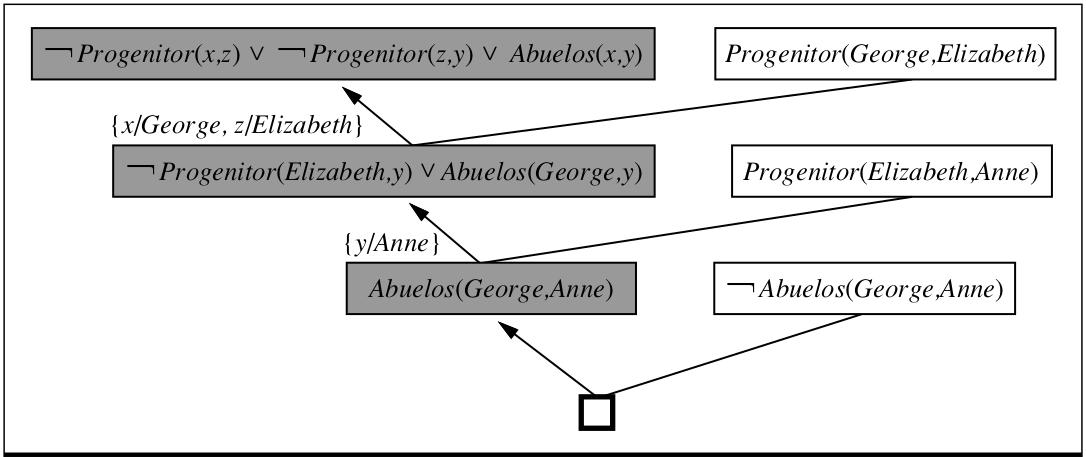
\includegraphics[width=0.8\textwidth]{./section3/fig9.png}
				\end{figure}
				
			\subsection{Hacer descubrimientos con la programación lógica inductiva}
				Un procedimiento de resolución inversa que invierte completamente la estrategia de resolución es, en principio, un algoritmo completo para el aprendizaje de teorías de primer orden. Es decir, si alguna Hipótesis desconocida genera un conjunto de ejemplos, un procedimiento de resolución inversa puede generar Hipótesis a partir de ejemplos.
				
				Esta observación sugiere una posibilidad interesante: suponga que los ejemplos disponibles incluyen varias trayectorias de cuerpos cayendo. ¿Podría un programa de resolución inversa ser teóricamente capaz de inferir la ley de la gravedad? Claramente la respuesta es que sí, ya que la ley de la gravedad permite explicar los ejemplos, dada una base matemática adecuada. De forma similar, podemos imaginar que el electromagnetismo, la mecánica cuántica y la teoría de la relatividad también pertenecen al ámbito de los programas de ILP. Por supuesto, se puede decir que también están al alcance de un mono con una máquina de escribir; todavía necesitamos heurísticas mejores y nuevas formas de estructurar el espacio de búsqueda.
				
				Algo que los sistemas de resolución inversa pueden hacer por nosotros es inventar nuevos predicados. Esta capacidad a menudo parece algo mágica, ya que normalmente parece que los computadores ``trabajan sólo con lo que se les da''. De hecho, los nuevos predicados se generan directamente a partir de los pasos de resolución inversa. El caso más simple aparece cuando tomamos como hipótesis dos nuevas cláusulas $C_{1}$ y $C_{2}$, dada una cláusula $C$. La resolución de $C_{1}$ y $C_{2}$ elimina un literal que las dos cláusulas comparten; a partir de aquí, es bastante posible que el literal eliminado contenga un predicado que no aparezca en $C$. Por ello, cuando se trabaja hacia atrás, una posibilidad es generar un nuevo predicado a partir de reconstruir el literal que falta.
				
				\begin{figure}[h]
					\centering
					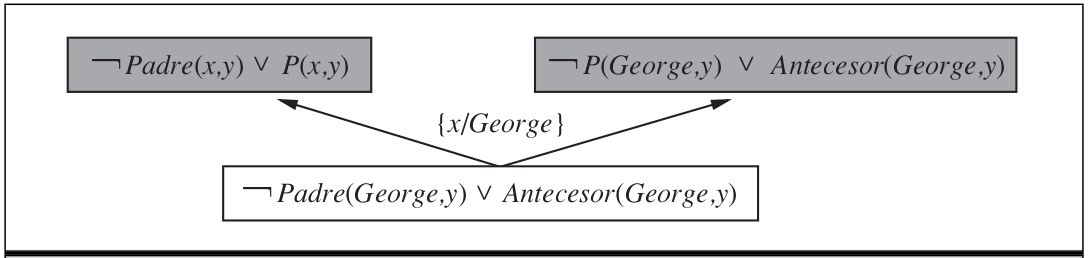
\includegraphics[width=0.8\textwidth]{./section3/fig10.png}
				\end{figure}
				Ejemplo en el cual el nuevo predicado $P$ se genera en el proceso de aprendizaje de la definición de Antecesor. Una vez generado, $P$ se puede usar en pasos posteriores de resolución inversa. Por ejemplo, un paso posterior podría tomar como hipótesis $Madre(x, y) \Rightarrow P(x, y)$. Por ello, el nuevo predicado $P$ tiene su significado restringido por la generación de hipótesis relacionadas con él. Otro ejemplo podría llevarnos a la restricción $Padre(x, y)\Rightarrow P(x, y)$. En otras palabras, el predicado $P$ es lo que hemos denominado la relación Progenitor. Como mencionamos anteriormente, la invención de nuevos predicados puede reducir el tamaño de la definición del predicado meta. Por lo tanto, incluyendo la habilidad de inventar nuevos predicados, los sistemas de resolución inversa pueden resolver a menudo problemas que es inviable resolver con otras técnicas.
				
				Algunas de las revoluciones más trascendentes que se han producido en la ciencia
vienen de la invención de nuevos predicados y funciones, por ejemplo, la invención de la aceleración de Galileo, o la invención de la energía térmica de Joule. Una vez que estos términos están disponibles, el descubrimiento de nuevas leyes se convierte en una tarea (relativamente) fácil. La parte difícil recae en darse cuenta de que alguna nueva entidad, con una relación específica con entidades existentes, permitiría que un cuerpo entero de observaciones sea explicado de una forma más simple y con teorías más elegantes de las que previamente existían.

				Hasta ahora, los sistemas ILP no han hecho descubrimientos al nivel de Galileo o Joule, pero sus descubrimientos han sido juzgados como publicables en la literatura científica. Por ejemplo, en la revista Journal of Molecular Biology, Turcotte et al. (2001) describen el descubrimiento automático de reglas para el pliegue de proteínas usando el programa P ROGOL de ILP. Muchas de las reglas descubiertas por P ROGOL podrían haber sido derivadas a partir de principios conocidos, pero la mayoría no habían sido previamente publicadas como parte de una base de datos biológicos estándar. En trabajos relacionados, Srinivasan et al. (1994) trataban el problema de descubrir reglas basadas en la estructura molecular para la mutación de componentes nitroaromáticas. Estas componentes se encontraron en gases de automóviles. Para el 80 por ciento de las componentes de una base de datos estándar, es posible identificar cuatro características importantes. La regresión lineal sobre estas características mejora a ILP. Para el restante 20 por ciento, las características por separado no pueden predecirse, e ILP identifica relaciones que le permiten mejorar la regresión lineal, las redes de neuronas y los árboles de decisión. King et al. (1992) mostró cómo predecir la eficacia terapéutica de varias drogas a partir de su estructura molecular. En todos estos ejemplos se observa que tanto la habilidad de representar relaciones como el uso de conocimiento básico contribuyen al alto rendimiento de ILP. El hecho de que las reglas encontradas por ILP puedan ser interpretadas por los humanos contribuye a la aceptación de estas técnicas tanto en revistas de Biología como en revistas de informática.

				ILP ha contribuido a otras ciencias además de la Biología. Una de las más importantes es el procesamiento del lenguaje natural, donde ILP se ha usado para extraer información relacional compleja a partir de un texto. 

				
\end{document}
			